\documentclass[12pt,a4paper]{article}
\title{%
  Labforsøk i rotasjonsmekanikk \\
  \large IFYKJT1001 - Fysikk/Kjemi \\
  }
\author{Gunnar Myhre, BIELEKTRO}

\usepackage[utf8]{inputenc}
\usepackage[norsk]{babel}
\usepackage{amsmath}
\usepackage{siunitx}

\usepackage{graphicx}
\graphicspath{ {./images} }

\setlength\parindent{0pt}

\begin{document}
  \maketitle
  \tableofcontents

  \section{Hensikt}
  Hensikten med dette forsøket er å få erfaring med å utføre fysiske
  eksperiment.  Vi skal få erfaring med teknikkar som er sentrale i labforsøk,
  slik som vurdering av systematiske eller tilfeldige feilkjelder, og utrekning
  av standardavvik. Vi skal også teste dei teoretiske verdiane frå
  rotasjonsmekanikken opp mot målte verdiar.

  \section{Teori}
  \subsection{Reint rullande gjenstand på skråplan}
  Vi har ein gjenstand som ligger i ro på eit skråplan med vinkel $\beta$. For $t=0$ starter
  kula å akselerere på grunn av gravitasjonskrafta. Vi antar at kula ikkje vil gli men vil
  rulle reint nedover rampa. Summen av kreftene i akselerasjonsretninga (langs rampa) er då
  \begin{equation}
    mgsin\beta - f_s = ma_x
  \end{equation}
  friksjonskrafta $f_s$ kan vi beskrive med Newtons andre lov på rotasjonsform
  \begin{equation}
    \Sigma \tau = I\alpha \rightarrow f_s = \frac{I\alpha}{r}
  \end{equation}
  Sidan gjenstanden ikkje glir eller spinner stemmer forholdet $a_x = \alpha r$ og
  $v_{CM} = \omega r$. Vi kan forenkle
  \begin{equation}
    mgsin\beta - f_s = ma_x \rightarrow a_x = \frac{mgsin\beta}{m + \frac{I}{r^2}}
    \rightarrow a_x = \frac{mgsin\beta}{m\left( 1 + \frac{I}{mr^2} \right)}
  \end{equation}
  Vi har lært at det er eit konstant forhold mellom den kinetiske energien knytta til
  rotasjon og translasjon
  \begin{equation}
    c = \frac{K_{rotasjon}}{K_{translasjon}} = \frac{\frac{1}{2}I\omega^2}{\frac{1}{2}Mv^2_{CM}}
  \end{equation}
  sidan vi antar at gjenstanden ruller reint kan vi forenkle
  \begin{equation}
    c = \frac{\frac{1}{2}I\omega^2}{\frac{1}{2}Mv^2_{CM}} \rightarrow
    c = \frac{Iv^2}{mr^2v^2} = \frac{I}{mr^2}
  \end{equation}
  vi kan nå substituere for $c$ og finne formel for akselerasjon
  \begin{equation}
    a_x = \frac{gsin\beta}{1+c}
  \end{equation}

  \subsection{Teoretiske verdiar}
  Den hule sylinderen har mål
  \begin{itemize}
    \item $r_{ytre} = 25\cdot10^{-3}[m]$
    \item $r_{indre} = 19\cdot10^{-3}[m]$
  \end{itemize}
  Vi velger $\beta = \ang{10.2}$ og finner verdiar for akselerasjon
  \begin{center}
    \begin{tabular}{|c|c|c|c|}
      \hline
      Gjenstand &  treghetsmoment($I$)  &  rotasjonskoeffisient ($c$)  &  
      akselerasjon ($a_x$) \\
      \hline
      &&&\\
      Massiv kule  &  $\frac{2}{5}MR^2$ &  $\frac{2}{5}$  &  $1,241[m/s^2]$ \\
      &&&\\
      \hline
      &&&\\
      Hul sylinder  &  $\frac{1}{2}M(r^2_i + r^2_y)$ &  
      $\frac{1}{2}\left( 1 + \left(\frac{R_i}{R_y}\right) ^2 \right)$  &  $0,972[m/s^2]$ \\
      &&&\\
      \hline
    \end{tabular}
  \end{center}

  \subsection{Standardavvik}
  Standardavvik er eit mål for spredninga av verdiane i eit datasett.
  For å finne standardavvik finner vi først gjennomsnittet av målingene
  \begin{equation}
    \bar{x} = \frac{x_1 + x_2 + ... + x_N}{N} = \sum_{i=1}^{N} \frac{x_i}{N}
  \end{equation}
  deretter finner vi standardavviket fom gjennomsnittet av gjennomsnitta.
  \begin{equation}
    \delta x = \sqrt{ \sum_{i=1}^{N} \frac{1x_i - \bar{x}) ^2}{N - 1}}
  \end{equation}

  \section{Metode}
  \begin{figure}
    \begin{center}
      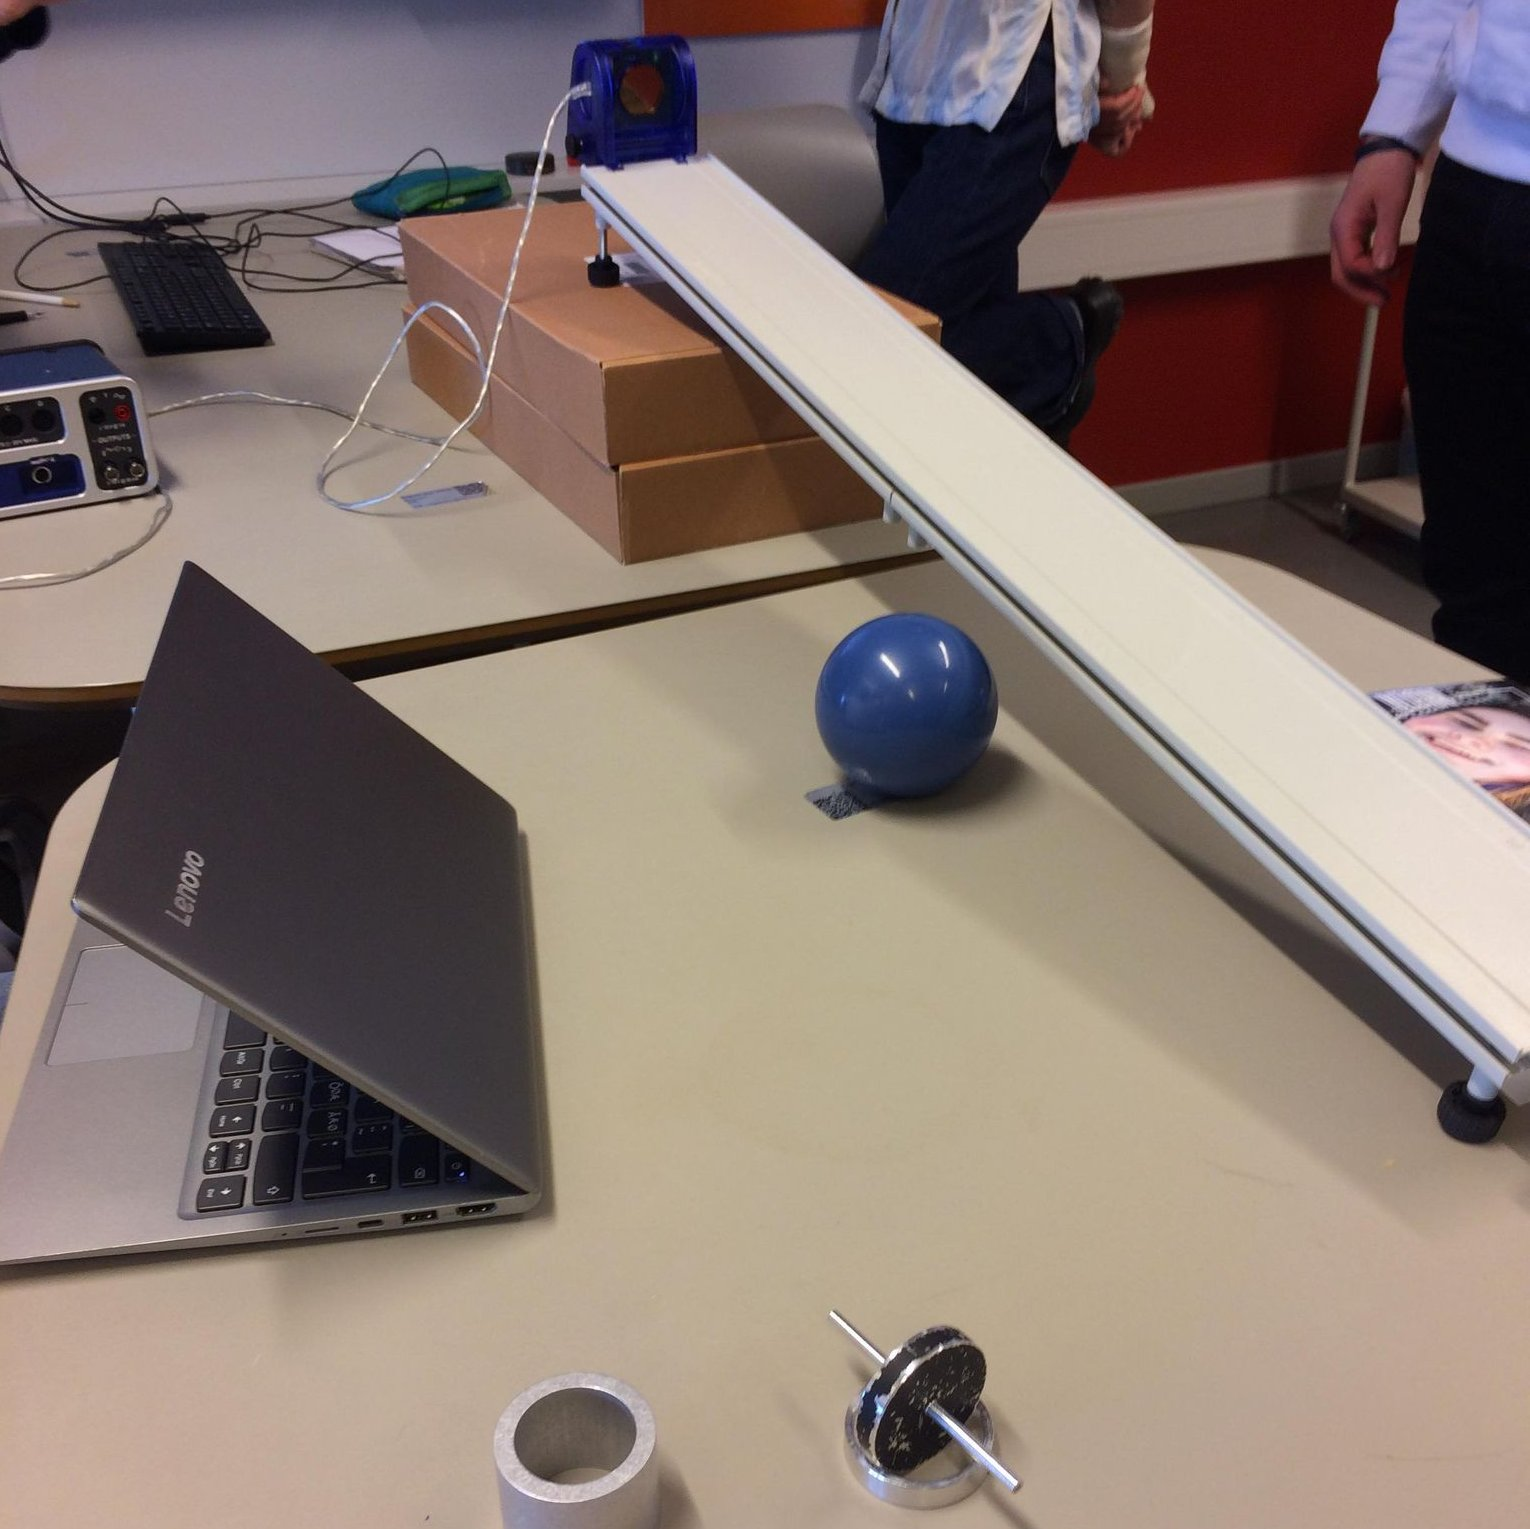
\includegraphics[scale=.1]{fylab1_oppsett.jpg}
      \caption{Eksperimentoppsett med rampe, bevegelsesmålar og gjenstandar.}
    \end{center}
  \end{figure}
  \subsection{Eksperimentoppsett}
  Vi bygger opp ei rampe ($L = 1\si{\meter}$) og justerer høgda til å bli $17,7 \si{\centi\meter}$.
  Dermed er helningsvinkelen $\beta = arcsin\left(\frac{17,7}{100} \right) = \ang{10,2}$.
  Gjenstandane slipper vi frå omtrent $15 \si{\centi\meter}$ under toppunktet på rampa.

  \subsection{Måleinstrument}
  Vi bruker ein \textit{PASCO PASPort (PS-2103A)}-bevegelsessensor plassert
  øverst på rampa for å måle gjenstandens posisjon over tid og dermed
  akselerasjonen. Sensoren er kopla til ein \textit{PASCO 850 Universal
  Interface}, og vi logger målingene på pc med \textit{PASCO Capstone}.

  \subsection{Valg av gyldig data}
  Når vi gjør eit sett av posisjonsmålinger hender det vi får støy i form av målinger langt utanfor
  rampa. Desse ser vi bort ifrå. Vi ser også bort ifrå målinger før gjenstanden starter å rulle,
  og etter gjenstanden har passert botnen av rampa. Vi velger den gyldige dataen med
  isoler-funksjonen i \textit{PASCO Capstone}.

  \begin{figure}
    \begin{center}
      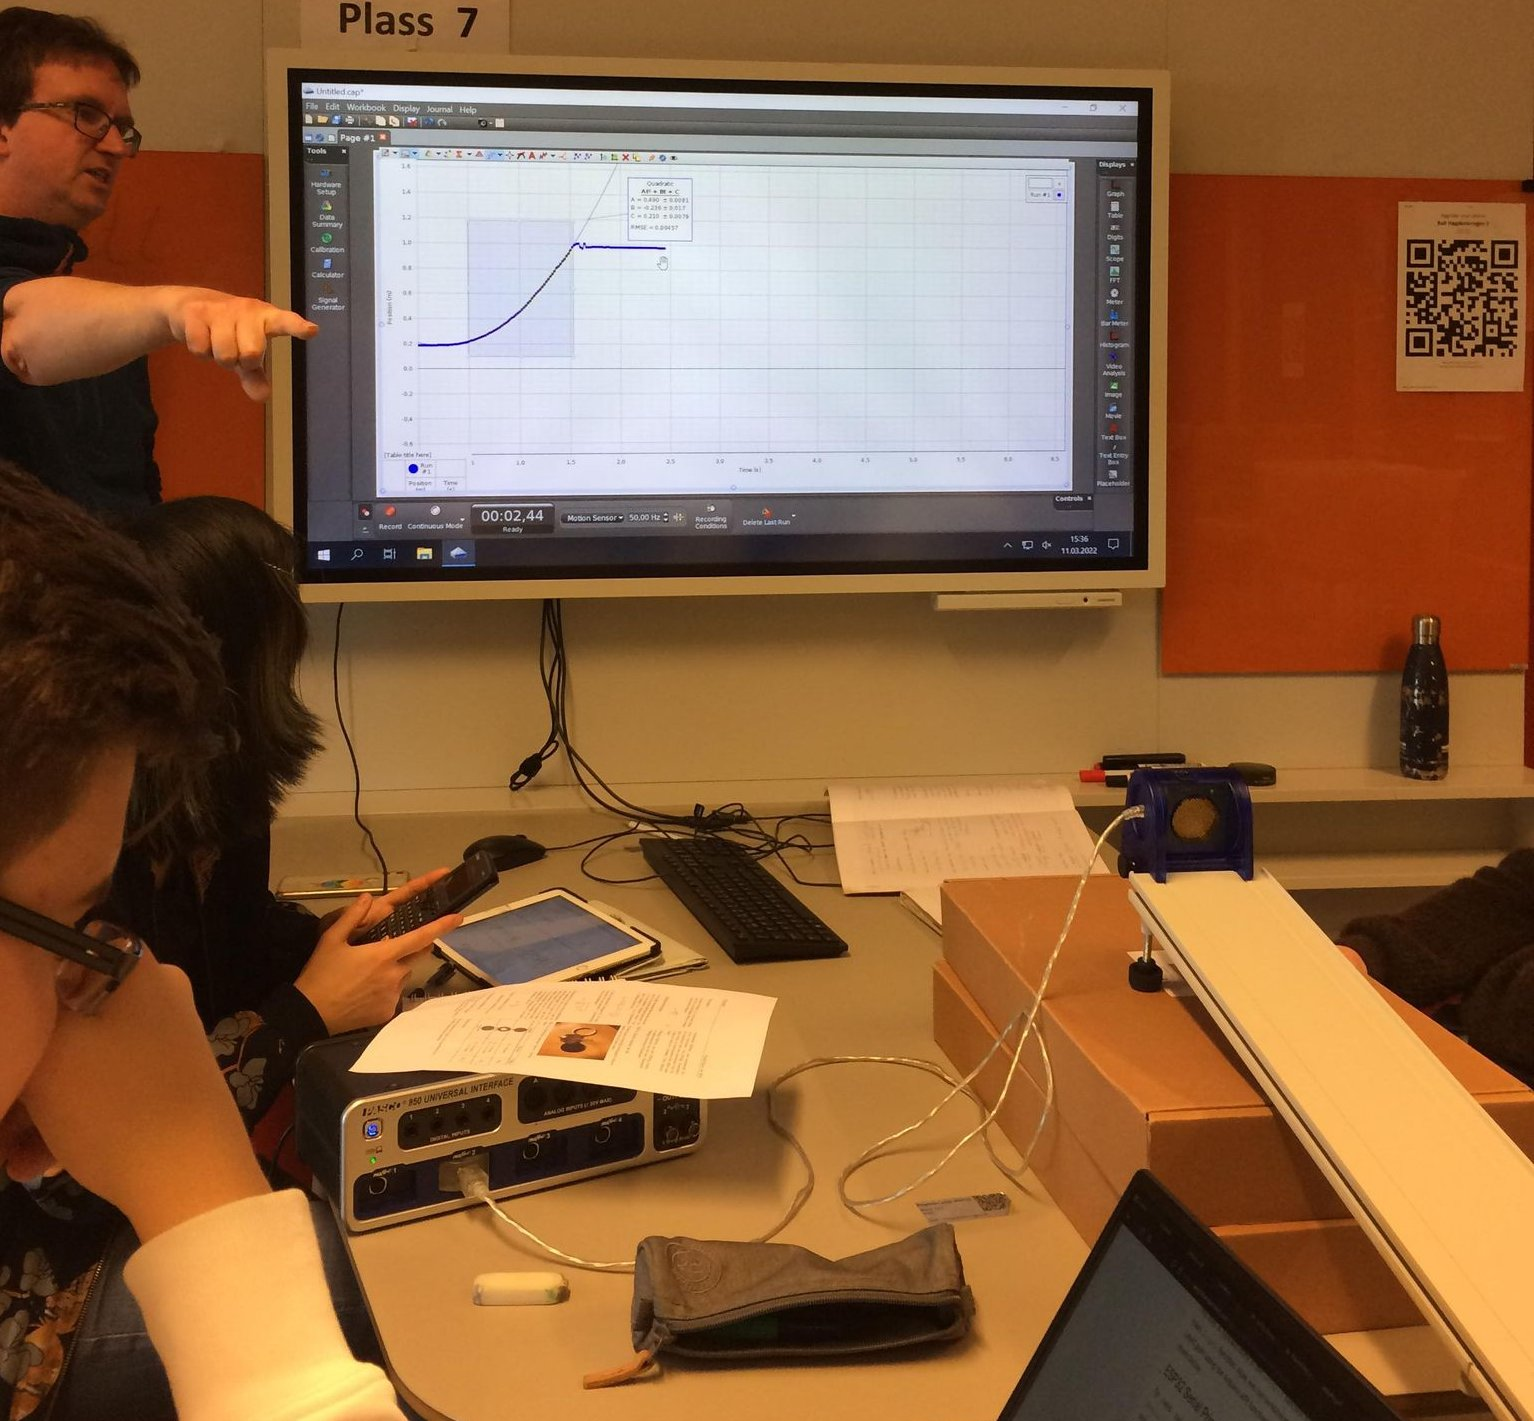
\includegraphics[scale=.1]{fylab1_reg.jpg}
      \caption{Bruk av \textit{PASCO Capstone} til å tolke posisjonsmålinger.}
    \end{center}
  \end{figure}

  \subsection{Utledning av akselerasjon frå eksperimentell data}
  Først finner vi ein passande kvadratisk regresjon til posisjonsmålingene vha.
  \textit{PASCO Capstone}. Så tidsderiverer vi dette utrykket to gonger for å finne
  akselerasjonen (i praksis gonger vi konstanten til andegradsleddet med to).


  \section{Resultater}
  \begin{center}
    \begin{tabular}{|c|c|c|c|}
      \hline
      Måling nr.: & hul sylinder & massiv kule  & einhet\\
      \hline
      1 &  $0.930$  &  $1,280$  &  $[\si{\meter}/\si{\second}^2]$\\
      \hline
      2 &  $0,992$  &  $1,246$  &  $[\si{\meter}/\si{\second}^2]$\\
      \hline
      3 &  $0.994$  &  $1,328$  &  $[\si{\meter}/\si{\second}^2]$\\
      \hline
      4 &  $1.050$  &  $1,274$  &  $[\si{\meter}/\si{\second}^2]$\\
      \hline
      5 &  $0.964$  &  $1,258$  &  $[\si{\meter}/\si{\second}^2]$\\
      \hline
       & & & \\
      \hline
      gjennomsnitt $\bar{x}$  &  $0,996$  &  $1,277$ &     $[\si{\meter}/\si{\second}^2]$\\
      \hline
      teoretisk verdi $a_{t}$  &  $0,972$  &  $1,241$ &    $[\si{\meter}/\si{\second}^2]$\\
      \hline
      standardavvik $\delta x$  &  $0,0290$  &  $0,0281$ & $[\si{\meter}/\si{\second}^2]$\\
      \hline
    \end{tabular}
  \end{center}

  \section{Diskusjon}
  Sidan vi ikkje har modellert luftmotstand i den teoretiske verdien ville vi
  forventa at målingene lå under teoretisk verdi. Vi ser av resultatene at det
  motsette er tilfelle. Dette skyldast nok ein eller fleire systematiske feilkjelder.
  \begin{itemize}
    \item Under valg av gyldig data la eg merke til at det ofte lå datapunkter
      (feilmålinger) eit lite stykke over den ellers jamne parabelkurva. Sidan
      desse låg nokså nært kurva vart dei med under utrekninga av regresjonen
      og bidro til å heve andregradsleddet.
    \item Vinkelen på rampa kan ha endra seg etter vi målte den. Ein liten endring
      frå $\ang{10.2} \rightarrow \ang{10.5}$ er nok til å heve teoretisk verdi til
      målt gjennomsnittsverdi. I praksis måtte vinkelen ha stege endå litt meir for å
      kompansere for luftmotstand.
    \item Vi kan ikkje utelukke at gjenstandane sklei i løpet av translasjonen.
  \end{itemize}

  \section{Konklusjon}
  Resultatene våre er innanfor rimelighetens grenser, og feilkjeldene skyldast
  at det tross alt var ei kort laboppgåve. Den viktigaste forbetringa ville
  vere å sette rampa ein meir stabil plass så vi ikkje dytta borti den. Det var
  interessant å samanlikne dei utrekna verdiane med målingene, og sjå korleis
  ein kan gjere regresjonar på målingsdatasett. Eg ser for meg at
  forsøksteknikk vil vere nyttig i meir reelle samanhengar i framtida.

\end{document}
